\chapter{Methodology}\label{ch:methodology}
Collaborative research projects such as Polifonia are confronted since the beginning with the question of how to organise the work in order to fulfil the objectives of the project and giving provide a unified view of the project outputs.
This is typically achieved with an \textit{integration} work package or task which as the goal of developing a software output in the form of a system, often referred to as "framework"~\cite{johnson1997frameworks} that incorporates WP outputs in a unified object, offered to the target community as an Open Source software.
However, such approach raised some concerns during the first Technical Board meeting. 
Particularly, the discussion converged into questioning the utility of software frameworks in satisfying the needs of the target communities.
Those concerns resonated a recent trend in software development communities\footnote{An interesting reading on some problems with frameworks can be found at \url{https://medium.com/@itmarketplace.net/the-problem-with-frameworks-1fafa148dbad}, accessed 18/05/2021}. 
Software frameworks are monolithic in nature, and this may impact the re-usability of its components in third-party applications, and the possibility to support applications in corner cases which were not originally considered by the framework developers. 
Such integrated tools provide a multiplicity of affordances in one user space reducing the ability of being effective for specific tasks\footnote{\url{http://cloudscaling.com/blog/cloud-computing/killing-the-storage-unicorn-purpose-built-scaleio-spanks-multi-purpose-ceph-on-performance/}, accessed 28/05/2021.}.
In addition, providing a framework increases the learning curve to new users, which need to enter the creators' mindset to approach the solution.
Finally, complex projects such as Polifonia target a variety of sub-domains, users, and scenarios. 
As a result, effective solutions will necessarily be heterogeneous.
These concerns, raised during the first Technical Board meeting, required us to approach the problem of collaborative development (and output design) in a different way.

The methodology used for the development of the pilots and the Polifonia ecosystem is inspired by agile software development methodologies \cite{collier2012agile}. 
Similar to those, our methodology focuses on \textit{``discovering requirements and developing solutions through the collaborative effort of self-organising and cross-functional teams and their customer(s)/end user(s)''}. 
This distributed, self-organised approach has several advantages, especially when confronted with a more traditional, waterfall-based model~\cite{benington1983production}:

\begin{itemize}
    \item Does not enforce specific non-functional requirements to any of the development teams, such as programming languages, libraries, or frameworks; therefore minimising the chances of writing large, monolithic systems that are hard to document and maintain (especially after the end of the project). % \todo{@all: add something about long-term sustainability? E.g. innovation task force in WP6}
    \item Identifies and reduces dependencies between different Pilots or WPs. By refusing to establish dependencies between the tasks of the WPs, it allows activities to progress in parallel but ensuring coherence within the framework of the project, under the WPs supervision
    \item It is feature-driven, and puts the requirements from the Pilots at the forefront of the development process, involving domain experts as co-creators from the start
    \item Allows for incremental and frequent software releases under the open-source mantra ``release early, release often'', to maximise the opportunity of getting feedback from the target community at early stage, and validate the output against core requirements at the early stage
    \item Increases decoupling and independence of components, since each component has autonomous value and can be used by and combined with other components (e.g. the Pilots and the Web Portal). 
    \item Increases opportunity for reuse of technical and scientific artefacts
    \item Maximise the sustainability of the outputs beyond the scope of the project, less effective components can be abandoned, without compromising the more successful ones
    \item Allows for a decentralised quality assurance process, where project-global metrics can be implemented in task-specific components
\end{itemize}

% \todo[inline]{[IMAGE: OVERVIEW OF THE COLLABORATIVE METHODOLOGY]}
\begin{figure}
    \centering
    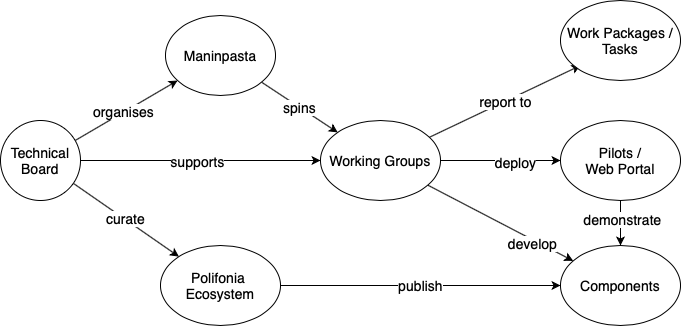
\includegraphics[width=1\textwidth]{images/Polifonia-D1.3-Methodology.png}
    \caption{Overview of the collaborative methodology}
    \label{fig:methodology}
\end{figure}
An overview of the methodology is presented in Figure~\ref{fig:methodology}.
The main ingredients of our methodology are: (a) collaborative workshops; (b) agile working groups; (c) work packages; and (d) pilots.

In Polifonia, the activity is bootstrapped in \textit{collaborative workshops}, named \textit{Maninpasta}\footnote{From the Italian, translates literally as "with the hands in the dough". Metaphorically, the meaning resembles the English "getting one's hands dirty".} where technology and domain experts meet to discuss themes of interest, inspired by the Pilots. 
The workshop starts with an open session where participants can propose relevant themes. 
Then, participants distribute to the various groups by following their personal interest.
Often (but not necessarily), this is in line with the person role in the project.
At the end of the workshop, groups report on the work done. 
Eventually, the workshop spins the creation of cross-functional teams that continue as independent \textit{agile working groups}. However, this is not mandatory, and some groups discussion may not survive beyond the workshop. Often, these groups split and individual participants join other teams.

\textit{Working groups} are targeted to develop specific aspects such as develop requirements of a given Pilot, or design the technical solution to solve a certain problem.
working groups produce concrete outputs as components of the Polifonia Ecosystem.
For example, the first Maninpasta workshop lead to the activities MusicAnnotation\#1\footnote{\url{https://github.com/polifonia-project/stories/issues/12}}, MockupDesign\#1\footnote{\url{https://github.com/polifonia-project/stories/issues/10}}, OntologyDesign\#1\footnote{\url{https://github.com/polifonia-project/stories/issues/7}}, and  BuildingKG\#1\footnote{\url{https://github.com/polifonia-project/stories/issues/6}}, among others.
Details of the co-creation process happening in the working groups can be found in Deliverable D1.1 - Roadmap and pilot requirements.

These cross-functional teams are organised by the various technology-oriented \textit{Work Packages} (WP2 --knowledge graphs--, WP3 --music pattern discovery--, WP4 --text pattern discovery-- and WP5 --user interfaces--). 
Work package leaders have the duty of matching the content of the working groups with WP tasks and organise the scientific output coherently with the WP goals.

The customers/end users are represented by the various \textit{Pilots} (WP1), which constitute the \textit{demand}, that the technical output under development in the working groups (the \textit{offer}) aims at addressing. 
Therefore, WPs and Pilots are orthogonal and complementary views on how the consortium org.
Finally, it is the role of the Technical Board to ensure the quality of the assets produced and organise them into an Ecosystem of reusable components.

Our methodology inherits several benefits from agile methodologies, while making it converge with the project framework in a two-fold way:
\begin{itemize}
    \item \textbf{Bottom-up approach}. Component development, and especially the gathering, documentation and maintenance of requirements for such components, are managed by the working groups. This is a hackathon-like, grassroots approach that periodically ensures interaction between requirement providers in the Pilots, and software development teams in the technological WPs.
    \item \textbf{Top-down approach}. WP leaders and TB members ensure that the bottom-up approach is aligned and converges, to the extent possible, to the goals established by Polifonia GA. This includes the establishment of WP checkpoints (e.g. previous to a milestone or a deliverable); and explicit breakdowns and plannings of how features, commits, releases, etc. align with the planning of WPs and their tasks. The TB synchronises and complements this top-down supervision in conjunction with the WP and Task leaders.
\end{itemize}
In addition, our process adds the following procedures:

\begin{enumerate}
    \item \textbf{Component development life-cycle}. Components stem from working groups and are developed in the collaborative platform (GitHub). Each component is developed in a code repository. Issue tracking and versioning ensure the development process is monitored and shared with the community that is invited to raise issues and discuss solutions. When the work towards a features is complete, the repository owner plans for a release.
    \item \textbf{Sign-off release}. The release of new software components into the ecosystem must follow a code review, involving one or two code reviewers from a different team from the one that carried out the development. Specifically, the repository owner prepares a release candidate, then reviews are initiated and monitored via the Issue tracker on GitHub. When complete, the current state of the repository is marked for release, and the actual release is produced. % More specifically, this happens when a \emph{development branch} requests a \emph{merge with its main branch} via a \emph{pull request}; such a pull request must include a code review request to the aforementioned external reviewers \todo{@all: check this is how we want to do it?}
    \item \textbf{Licencing}. Releases need to have associated explicit licencing information, which is particular important to maximise the dissemination of project outputs. The TB recommends the delivery of Open Source software published with a commercial-friendly Apache Licence 2.0. However, consortium members can choose to alternative licences, after consultation with the TB and according to the guidelines of the GA.
    \item \textbf{Polifonia Ecosystem}. Components' releases are collected, annotated, and organised in the Polifonia Ecosystem, which constitutes the unified entry-point to the technical outputs of the project.
\end{enumerate}

% \todo[inline]{IMAGE: COMPONENTS' LIFECYCLE}

% \todo{Outline}
% WP and Pilots are Orthogonal 
% Goal: identify and reduce dependencies 
% Increase opportunity for reuse (scientific / technical) 
% Agile, feature-driven 
% Incremental releases: "release early, release often” 
% Decoupling / independence (each component has an autonomous value but *can* also be used with others, as exemplified in Pilots and Web Portal) 
% Quality assurance 
% Sign-Off release process, involving one or two code reviewers from another team 
% Component development lifecycle 
% Methodology Two-fold: 
% (a) Bottom-Up: Maninpasta / hackatons grassroots approach 
% (b) Top-Down: Checkpoint during WP, relation with WPs, tasks, etc … / Checkpoint on TB 